\section{Create a modelling project}

%%%%
%%%%
%%%%
\begin{frame}{What you need to start this tutorial}

\smallblock{Needed data}

	\begin{enumerate}
		\item Ecore Meta-model (here we use maps.ecore).
		\item Images and icons for elements (given images folder).
		\item Eclipse EMF.
		\item Install Sirius in Eclipse .
	\end{enumerate}

\end{frame}	

%%%%
%%%%
%%%%
\begin{frame}{Create a Modelling project}

\smallblock{step \nextstep : Create an empty modelling project}

	\begin{enumerate}
		\item File \ra New \ra Empty modelling project.
		\item Copy {\it maps.ecore} and {\it images/} into the new project.		
	\end{enumerate}

\end{frame}

%%%%
%%%%
\begin{frame}{Create an EMF generator model}

\smallblock{step \nextstep: Create an EMF Generator Model}

	\begin{enumerate}
		\item maps.ecore Right \ra New \ra EMF Generator Model
	\end{enumerate}

	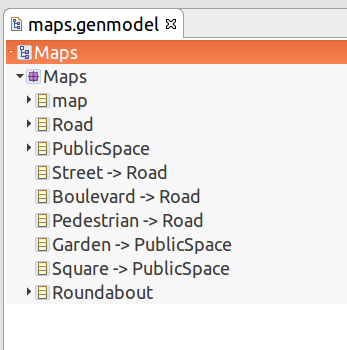
\includegraphics[scale=0.3]{figs/genmodel.png}

\end{frame}


%%%%
%%%%
\begin{frame}{Generate the code of the meta-model}

\smallblock{step \nextstep: Generate the code of the meta-model}

	\begin{enumerate}
		\item in maps.genmodel \ra Maps Right \ra generate all
	\end{enumerate}

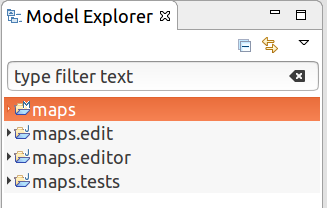
\includegraphics[scale=0.3]{figs/workspace1.png}

\end{frame}

%%%%
%%%%
\begin{frame}{Run maps project as a new Eclipse}

\smallblock{step \nextstep: run as new eclipse application}

	\begin{enumerate}
		\item Run \ra Run as \ra Eclipse Application		
	\end{enumerate}

\end{frame}

%%%%
%%%%
%%%%
\begin{frame}{Create a first instance of the meta-model}

\smallblock{step \nextstep: Create maps Model}

	\begin{enumerate}
		\item In runtime Eclipse: Create a Sirius Project (eg. test)
		\item New \ra maps Model (eg. mapVienna.maps)
		\item Create some elements in mapVienna.maps (new Street, Garden ...)
	\end{enumerate}

	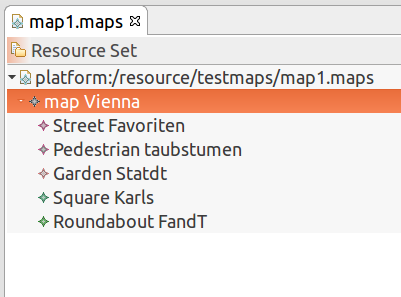
\includegraphics[scale=0.3]{figs/mapVienna1.png}

\end{frame}

\section{Create a Viewpoint Specification project}

%%%%
%%%%
%%%%
\begin{frame}{Create a Viewpoint Specification Project}

\smallblock{step \nextstep: Create a Viewpoint Specification Project}

	\begin{enumerate}
		\item In runtime Eclipse: New \ra Viewpoint Specification Project (eg. maps.design)
		\item a Viewpoint Specification Model is automatically created (maps.odesign)
		\item Rename the root element of .odesign file and set it to maps.
		\item Do the same for the viewpoint element.
	\end{enumerate}

	\centering
	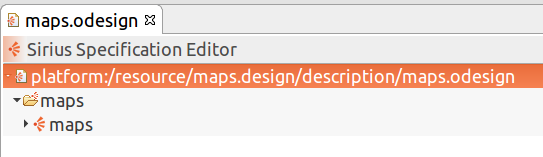
\includegraphics[scale=0.3]{figs/odesign1.png}

\end{frame}

%%%%
%%%%
%%%%
\begin{frame}{Create a new Diagram Description}

\smallblock{step \nextstep: Create a new Diagram description}

	\begin{enumerate}
		\item In maps.odesign: maps viewpoint right click \ra new representation \ra new Diagram Description
		\item set the properties of the created element: id = map, Domain class= maps.map (the root class of the meta-mode)
		\item Now you can start the creation of you editor
	\end{enumerate}

\end{frame}

%%%%
%%%%
%%%%
\begin{frame}{Test you editor}

\smallblock{step \nextstep: Create a representation}

	\begin{enumerate}
		\item In test project: expand .maps model and right click of root element (use modelling perspective)
		\item New representation \ra other \ra select map
		\item Now you can open map diagram (normally it is empty because no element was created)
	\end{enumerate}

\end{frame}

%%%%
%%%%
%%%%
